\documentclass[11pt,border=5pt]{standalone}
\usepackage{fontspec}
\setmainfont{cmunrm.otf}[BoldFont=cmunbx.otf,ItalicFont=cmunti.otf,BoldItalicFont=cmunbi.otf]
\usepackage{amsmath}
\usepackage{unicode-math}
\setmathfont{NewCMMath-Regular.otf}
\usepackage{tikz}
\usetikzlibrary{arrows.meta,patterns,angles,quotes}
\begin{document}
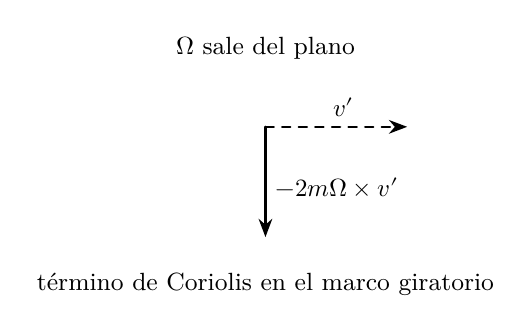
\begin{tikzpicture}[>=Stealth,font=\small,line cap=round,line join=round]
\draw[->,thick,dashed] (0,0) -- (1.8,0) node[pos=0.55,above] {$v\prime$};
\draw[->,thick] (0,0) -- (0,-1.4) node[pos=0.55,right] {$-2m\Omega\times v\prime$};
\node at (0,1) {$\Omega$ sale del plano};
\node at (0,-2) {término de Coriolis en el marco giratorio};

\end{tikzpicture}
\end{document}
